\begin{figure}[h]
    \centering
    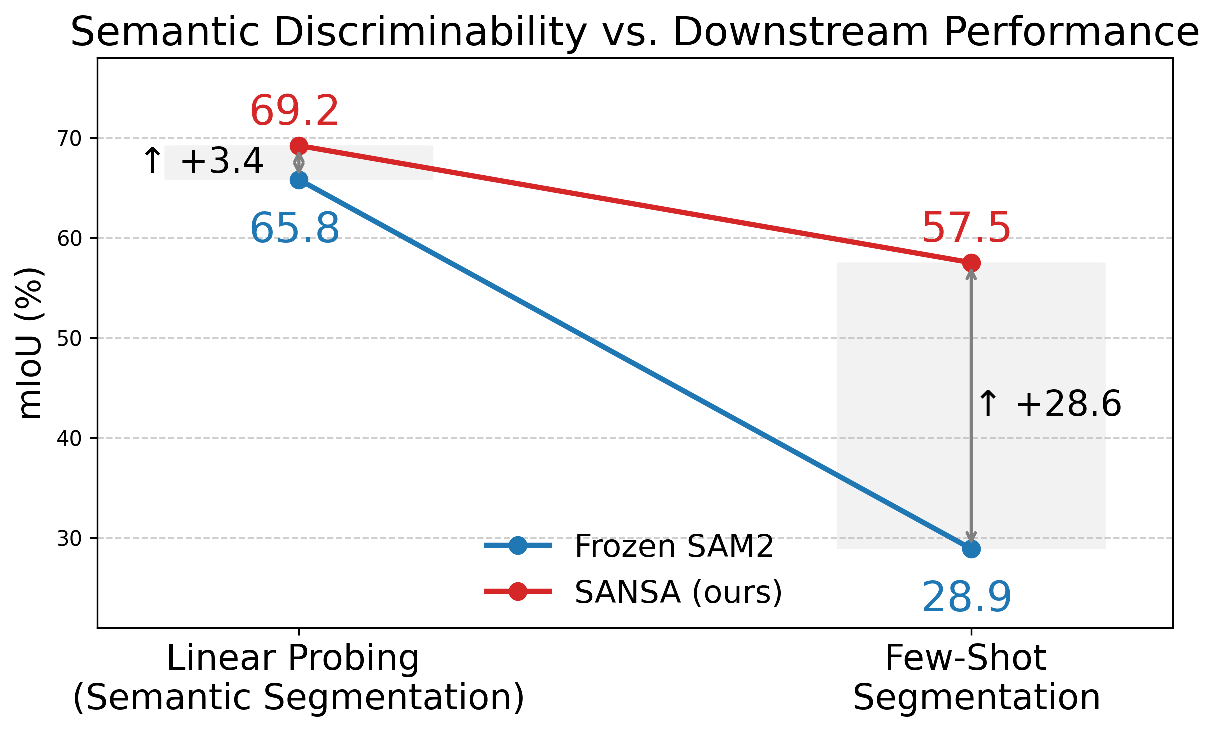
\includegraphics[width=.7\textwidth]{images/sam2_miou.pdf}
    \caption{Left: \textbf{Linear probing} for Semantic Segmentation on a fold of COCO-20$^i$, comparing frozen \sam{} and \ours{} (trained on a disjoint class set). Right: \textbf{Few-shot segmentation performance on the same set of data.} 
    Despite poor performance on few-shot segmentation, a simple linear layer (\textit{cf} linear probing) can learn to discriminate semantic-classes from \sam{} frozen features. These results, together, suggest the presence of semantic structure, albeit entangled with other signals.
    \label{fig:probing}}
\label{fig:linear_probe}
\end{figure}
